\chapter{Technical analysis} \label{technical analysis}

This chapter explains the technical requirements for the POC (proof-of-concept) project, which is central to the analysis of the research question of the thesis.
The chapter also lists our options for the technical implementation as well as rationalizes the decisions made.

\section{High level specification}

% datan voi pitää PoC:ssa yksinkertaisena, esimerkiksi asiakkaiden vastaanottoajat (nimi, hetu, pvm, vastaanottajan tiedot ja toimipisteen tiedot). Näitä sitten muutama miljoona skriptillä. 
% Kryptauksen kysymykset ovat mielestäni juuri niitä avainasioita, joita olisi työssäsi hyvä käydä läpi
% Miten luettelemasi tavat vaikuttavat suorituskykyyn, ohjelmiston ja ympäristöjen toteutukseen, ylläpidettävyyteen ja selkeyteen. 
% Tuovatko ne oikeasti lisäturvaa.
% PoC:ssa toteutettavaksi voisi valita yhden, joka paperilla osoittautuu parhaimmaksi vaihtoehdoksi.
% Tai sitten tekee useamman toteutuksen ja tekee kovan vertailun. Ihan miten ajakäyttöösi ja työsi rakenteeseen vain parhaiten sopii.

The POC projects is built to replicate a close-to real world application for storing sensitive customer data.
The data stored is related to appointment times of any specific customer.
The application must be able to receive new appointment times and save them persistently.
It must also be able to load the state of the appointments.
All the actions are required to be fulfilled in a timely manner.
The appointment must store at least the following data
\begin{itemize}
    \item The customer's name
    \item The customer's social security number
    \item Date and time of the appointment
    \item Practitioner's name and basic info
    \item Location's name and basic info
\end{itemize}

The application must be available on the web and use an existing standard for interfacing with it.
Additional technical specifications are discussed in the next section.

\section{Technical specifications}

The application must support reading and writing data on practitioners and customers' appointments.
Preferably, the application provides REST-like endpoints for both types of data.
Each appointment must reference exactly one practitioner to whom the appointment is reserved.
All the data the application saves must be stored in a persisting PostgreSQL database.

The application must encrypt all data before it is sent to the database i.e. encryption at rest.
The master key for decrypting the data must be stored in a secure place, preferably inside the cloud provider's pre-made solution.

The application must be hosted inside the Google Cloud Platform's offering.
The products used can be chosen freely while considering the most practical option for the task, while preferring fully-managed options.

After the technical implementation of the application and the infrastructure are built, the performance of the application will be benchmarked with both encryption enabled and disabled.
This is likely to expose bottlenecks of the system, which will then be analyzed further to improve the performance of the application.

% Toteutuksen selkeys ja ylläpidettävyys tähän?
% Kuuluuko tekniseen speksiin vai tutkimuskysymykseen?

% Kirjottasko tähän miksi valittiin tietyt tekniikat?


% Mielestäni tähän sopivat syyt tekniikkojen valinnoille, voi toki olla myös oma alilukunsa tai sitten voi lisätä tämän aliluvun otsikkoon "and architectural decisions" tms.
% 
% Jos selkeydellä ja ylläpidettävyydellä viitataan näiden laatuattribuuttien arviointiin, niin tämä voi olla ehkä myöhemminkin?
%
% -SR

\section{Technology and architecture decisions}

The technological and architectural decisions are explained in this section.
The decisions were based on the specification of the POC project and based on solutions most commonly used in the industry.

The server application will be built with TypeScript running on top of Node.js.
TypeScript is a well-proven language for writing business critical applications using Node.js' large ecosystem of packages.
As the basis for the RESTful application, we will use Express: a minimal framework for building web applications.
The database for storing our patient data will be PostgreSQL.
The interface library for our database is pg-promise.
These technologies were selected because of their use in the business as well as their match with our specification.

Docker is used during development for ease of spinning up a local PostgreSQL database for development.
The server application will also be built into a custom Docker image for production.

For hosting the POC project we have decided to use Google Cloud Platform and its solutions most compatible with our technology requirements.
For hosting the Node.js application, GCP's \textit{Cloud Run} will be used.
Cloud Run is a fully-managed service for running containerized applications.
For hosting our application's Docker images, we will use GCP's \textit{Artifact Registry}.
Artifact Registry is a cloud-based solution for managing a Docker registry.
For managing our PostgreSQL database, GCP's \textit{Cloud SQL} is the technology of choice.
Cloud SQL is a fully-managed service for administering relational databases, and it supports PostgreSQL along with MySQL and SQL Server.

For managing our sensitive environment variables, GCP's \textit{Secret Manager} is the service selected.
Secret Manager promises to store sensitive secrets encrypted and secure.
For secure encryption and decryption of data, without customer accessible keys, we will use GCP's \textit{Cloud Key Management}.
The encryption strategy will be discussed in more detail in the coming sections.

For a real world use case, we might also need solutions for managing routing, domains and virtual private networks.
In our POC project, the Cloud Run application is connected straight to the internet using the GCP provided dynamic domain.
Another part of a real world application's infrastructure not included here is a user management solution.
This is also outside the scope of the POC project.
The infrastructure is visualized in figure \ref{fig:infrastructure}.

\begin{figure}[!htb]
\centering
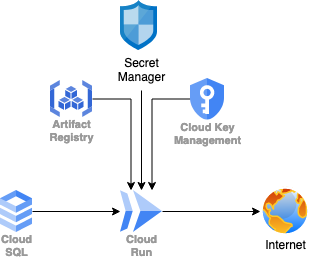
\includegraphics[scale=0.9]{infrastructure}
\caption{Visualization of the infrastructure in the Google Cloud}
\label{fig:infrastructure}
\end{figure}

\section{Cryptography options on Google Cloud}

Google Cloud Platform offers multiple solutions for encrypting data.
The easiest solution for implementing encryption with Google Cloud Platform is to let Google handle it automatically.
Google encrypts all of their customer data at rest by default, with zero configuration required by the developer.
This is done to avoid the possibility of a data breach allowing a malicious actor direct access to the plaintext data.
This encryption uses the same standards for hardened key management services that they use internally.
This system uses the AES-256 encryption standard.
\cite{googlecloud}

Besides GCP's encryption by default, developers can choose to encrypt their data with other options.
GCP's Cloud Key Management Service (KMS) is a solution for creating, using, rotating and managing cryptographic keys entirely on Google Cloud.
KMS can be used for example to provide customer-managed encryption keys (CMEK) for GCP's Cloud Storage or called by an API to encrypt any plaintext data.
Keys stored in KMS are designed to never leave Google servers making them theoretically impossible to be stolen if a malicious actor gains access to the system.
While KMS can be used to encrypt almost anything, it is built more for being the central key store in a multi-layer encryption architecture such as for storing the key encryption keys in an envelope encryption setup.
\cite{googlecloud}

GCP also provides the option for customer-supplied encryption keys (CMEK) for many of its products that encrypt data by default, such as Cloud Storage.
Google does not permanently store these type of keys, instead the key must be provided along with any operation call.
A cryptographic hash of the key is stored on Google server to validate the requests.
\cite{googlecloud}

The PostgreSQL database system has built-in support for multiple types of encryption.
A fully-managed PostgreSQL limits the developer's options a little, as they do not have access to encrypt the entire data partition by themselves.
However, encryption for specific columns using PostgreSQL's built-in pgcrypto-module is still possible.
The data can also be encrypted on the client side before it is sent to the database system.
\cite{postgresql}

% trade-off for column-level encryption:
% client can no longer query data based on that column
% workaround: hash and salt the same data and store in another column for lookups

Fully cloud-based applications cannot be considered end-to-end encrypted, as the cloud provider theoretically has access to the unencrypted data while it is processed.
The solution to this would be encrypting the data on the client-side before it is sent to the cloud provider.
This can be done either on-premises or on the user's client device.
% lähde?

\section{The encryption strategy used}

For the POC project, an additional layer of security on top of GCP's encryption by default is required to secure the patient data.
For this reason, we will encrypt all sensitive data on the server before it is written to the database.
Google Cloud Key Management System is our choice of technology for managing secrets.
However, we want to minimize the calls to the KMS API for cost reasons\footnote{Google bills us \$0.03 per 10 000 requests to the API.}
and to allow for extra scalability.
For these reasons, we will not encrypt the data itself with the KMS API, but instead employ envelope encryption.

A great option for strong implementation of envelope encryption is to have the key encryption keys never leave KMS.
The data encryption keys will be generated on the server per-request to encrypt the data itself locally.
The DEKs are encrypted using the KEKs via KMS.
This allows for calling KMS only once per fixed-length DEK instead of once per each variable-length database column to cut down the amout of KMS API calls.

In a production environment, the above option is preferred.
However, in our small-scale solution, with plans to stress test the encryption setup, the KEK will be stored encrypted in an environment variable.
% Muokkasin edeltävää virkettä, kannattaa tarkistaa -SR
The KEK will be encrypted via KMS and decrypted on application startup.
This cuts down on calling the KMS API even more and makes sure we will never be billed more than a dollar for our use of its API.
Realistically, this is also a security vulnerability, as the key has to be generated in plaintext outside KMS and is stored in plaintext inside the server application's memory.
For these reasons, this solution is not recommended for any real private and sensitive data.

The encryption of the data itself can be handled on the server application code or by the database itself via PostgreSQL's built-in pgcrypto.
For the POC application, we decided to encrypt the data on the application itself to remove the bottleneck created by having to make two queries to the database: one for the DEK and one for the data itself.
The decision was also made to allow for more research into implementing encryption.

For encrypting the data and wrapping the data encryption key, Node.js standard library's crypto-module was chosen.
This module includes a lot of useful cryptographical utilities for generating keys, and encrypting and decrypting data with multiple encryption algorithms.
\cite{nodejs}
For our POC project we will use the crypto-module for generating data keys and implementing AES-256 encryption.
We will use Google Cloud Key Management Service to decrypt our key encryption key on program startup.
